\chapter{TỔNG QUAN VỀ BÀI TOÁN VÀ CƠ SỞ DỮ LIỆU}
\label{chap:chuong1}

\section{Bối cảnh thực tiễn và tính cấp thiết của đề tài}
\label{sec:boi-canh}

Trong những thập kỷ gần đây, cùng với sự phát triển bùng nổ của hạ tầng viễn thông và các thiết bị di động thông minh, dịch vụ tin nhắn ngắn (Short Message Service --- SMS) đã trở thành một trong những phương tiện truyền thông phổ biến nhất trên phạm vi toàn cầu. Với ưu điểm vượt trội về tính tức thời, khả năng tiếp cận mọi thiết bị di động mà không phụ thuộc vào kết nối Internet tốc độ cao, tỷ lệ mở tin nhắn thực tế lên tới trên 95\% trong vòng 3 phút đầu tiên sau khi nhận, SMS luôn được lựa chọn làm kênh liên lạc trọng yếu trong các lĩnh vực tài chính, ngân hàng, thương mại điện tử, dịch vụ công và y tế.

Tuy nhiên, song hành cùng sự tiện lợi to lớn đó, dịch vụ SMS cũng đang phải đối mặt với nguy cơ bị xâm hại nghiêm trọng bởi vấn nạn tin nhắn rác (SMS Spam). Không chỉ đơn thuần là các tin nhắn quảng cáo hàng hóa, bất động sản, dịch vụ cho vay tín dụng đen gây phiền toái cho người dùng cá nhân và tiêu hao băng thông của các nhà cung cấp dịch vụ mạng viễn thông, tin nhắn rác ngày nay đã biến tướng thành công cụ nguy hiểm của các tổ chức tội phạm mạng có tổ chức. Các thủ đoạn lừa đảo phổ biến bao gồm:
\begin{itemize}
    \item \textbf{Phát tán liên kết lừa đảo (Smishing/Phishing):} Tin nhắn giả mạo các ngân hàng thương mại, cổng thanh toán hoặc cơ quan bảo hiểm xã hội yêu cầu người dùng truy cập vào các website mạo danh để đánh cắp thông tin thẻ tín dụng, mã định danh cá nhân và mật khẩu đăng nhập.
    \item \textbf{Dụ dỗ gọi điện tới các đầu số dịch vụ thu phí cao (Premium-rate numbers):} Tin nhắn thông báo trúng thưởng lớn, bưu kiện thất lạc hoặc tin nhắn khẩn cấp yêu cầu người nhận gọi lại vào các số điện thoại lạ có cước phí viễn thông rất đắt để chiếm đoạt cước phí.
    \item \textbf{Cài cắm mã độc (Malware injection):} Dẫn dụ người dùng tải về các ứng dụng độc hại nhằm chiếm quyền điều khiển thiết bị di động, tự động đọc mã xác thực OTP ngân hàng hoặc biến máy nạn nhân thành máy trạm phát tán tin rác diện rộng (Botnet).
\end{itemize}

Trước làn sóng tấn công ngày càng gia tăng, các phương pháp bảo vệ truyền thống như lập danh sách đen (Blacklist) số điện thoại gửi hoặc áp dụng các bộ luật tĩnh (Rule-based filtering) đã hoàn toàn bộc lộ những hạn chế cố hữu. Những kẻ phát tán tin rác dễ dàng vượt qua danh sách đen bằng cách sử dụng các SIM rác dùng một lần, dịch vụ gửi tin nhắn giả mạo địa chỉ (SMS Spoofing) hoặc biến tấu chính tả từ ngữ để qua mặt các luật kiểm tra từ khóa cố định. Do đó, việc xây dựng một hệ thống phân loại tin nhắn rác tự động, ứng dụng các mô hình học máy hiện đại có khả năng tự động học hỏi các quy luật từ dữ liệu lớn và thích ứng linh hoạt với các biến thể tin nhắn mới là một yêu cầu kỹ thuật vô cùng cấp thiết, mang ý nghĩa to lớn cả về mặt lý luận lẫn ứng dụng thực tiễn.

\section{Mục tiêu nghiên cứu và phạm vi đề tài}
\label{sec:muc-tieu}

Được triển khai trong khuôn khổ học phần \textbf{Nhập môn Học máy (FIT4013)} do Khoa Công nghệ Thông tin --- Trường Đại học Đại Nam tổ chức, Đề tài 3: \textit{“Phân loại tin nhắn rác (SMS Spam Collection)”} được Nhóm 13 định hướng thực hiện với các mục tiêu trọng tâm sau:

\begin{enumerate}
    \item \textbf{Làm chủ quy trình học máy toàn diện cho dữ liệu văn bản:} Xây dựng một quy trình học máy chuẩn mực và khép kín từ khâu thu thập dữ liệu thô, khám phá thống kê (EDA), tiền xử lý văn bản, trích xuất và biến đổi đặc trưng, đóng gói pipeline tự động, tối ưu hóa siêu tham số đến đánh giá kiểm nghiệm và phân tích lỗi chuyên sâu.
    \item \textbf{Thiết kế và kiểm chứng các phương án xử lý dữ liệu thực nghiệm:} So sánh một cách có kiểm soát 3 mức độ tiền xử lý văn bản (từ dữ liệu thô đến chuẩn hóa có chủ đích bảo toàn tín hiệu và loại bỏ từ dừng) cùng 4 không gian biểu diễn đặc trưng (Bag-of-Words và TF-IDF kết hợp với unigram và bigram), nhằm làm sáng tỏ tác động của cách thức tiền xử lý đến hiệu năng mô hình.
    \item \textbf{Nghiên cứu đối sánh ba thuật toán học máy cốt lõi:} Lựa chọn và thực thi ba thuật toán phân loại tiêu biểu đã được học trong chương trình:
    \begin{itemize}
        \item Thuật toán xác suất thống kê: \textbf{Multinomial Naive Bayes (MNB)};
        \item Thuật toán dựa trên khoảng cách và không gian hình học: \textbf{K-Láng giềng gần nhất (K-Nearest Neighbors --- K-NN)};
        \item Thuật toán dựa trên cấu trúc luật và lý thuyết cây quyết định: \textbf{Cây quyết định (Decision Tree --- DT)}.
    \end{itemize}
    \item \textbf{Đảm bảo tính nghiêm ngặt về phương pháp luận và kiểm soát rò rỉ dữ liệu (Data Leakage):} Thiết kế quy trình phân tách dữ liệu hold-out và thẩm định chéo k-fold nghiêm ngặt, trong đó toàn bộ quá trình học tham số (từ vựng, trọng số IDF, min/max) chỉ được thực hiện trên tập huấn luyện của từng fold.
    \item \textbf{Đánh giá đa chiều và phân tích lỗi chi tiết:} Sử dụng hệ thống độ đo toàn diện gồm Accuracy, Precision, Recall, F1-score, ma trận nhầm lẫn và diện tích dưới đường cong ROC (ROC-AUC), với sự ưu tiên tuyệt đối cho F1-score của lớp thiểu số (Spam). Đi sâu phân tích từng trường hợp dự đoán sai để làm sáng tỏ các điểm mù của thuật toán.
    \item \textbf{Hiện thực hóa sản phẩm ứng dụng (Demo Application):} Xây dựng giao diện web demo trực quan tương tác bằng Streamlit và công cụ dòng lệnh CLI, tích hợp khả năng giải thích quyết định của mô hình (Explainable AI) phục vụ trình diễn và bảo vệ đồ án.
\end{enumerate}

Về phạm vi đề tài, nghiên cứu tập trung giải quyết bài toán phân loại nhị phân (Binary Classification) trên bộ dữ liệu chuẩn tiếng Anh SMS Spam Collection. Các kết luận và đánh giá thực nghiệm được rút ra trực tiếp từ dữ liệu thực tế và các mô hình học máy được triển khai trong khuôn khổ này.

\section{Giới thiệu bộ dữ liệu SMS Spam Collection}
\label{sec:dataset}

Bộ dữ liệu thực nghiệm được sử dụng trong đề tài là \textbf{SMS Spam Collection v.1}, một trong những tập dữ liệu chuẩn mực và được trích dẫn nhiều nhất trong cộng đồng nghiên cứu xử lý ngôn ngữ tự nhiên và học máy quốc tế. Tập dữ liệu này được xây dựng bởi các nhà nghiên cứu Tiago A. Almeida, José María Gómez Hidalgo và Akibo Yamakami (công bố năm 2011) và hiện được lưu trữ công khai trên kho dữ liệu danh tiếng của Đại học California, Irvine (UCI Machine Learning Repository).

\subsection{Nguồn gốc và giấy phép sử dụng}
Theo tài liệu công bố chính thức từ nhóm tác giả và tập tin đặc tả đính kèm \texttt{readme\_dataset.txt}, dữ liệu được tổng hợp và đối soát cẩn trọng từ các nguồn công khai, hợp pháp, đảm bảo tính đa dạng và trung thực của tin nhắn SMS di động:
\begin{enumerate}
    \item Nguồn Grumbletext: Diễn đàn trực tuyến của Vương quốc Anh nơi người dùng di động công khai phản ánh và trích dẫn các tin nhắn rác nhận được (đóng góp 425 tin nhắn rác spam).
    \item Luận án tiến sĩ của Caroline Tagg (Đại học Birmingham, Anh): Tập ngữ liệu 2.950 tin nhắn cá nhân hợp lệ (ham) do người dùng tại Anh tự nguyện đóng góp cho mục đích nghiên cứu ngôn ngữ học.
    \item Kho ngữ liệu NUS SMS Corpus (Đại học Quốc gia Singapore): Một tập hợp 1.902 tin nhắn SMS của sinh viên và người dùng di động tại Singapore đóng góp cho phòng nghiên cứu NLP.
    \item Ngữ liệu SMS Spam Corpus v.0.1 Big: Đóng góp 450 tin nhắn rác và 1.002 tin nhắn hợp lệ thu thập phục vụ nghiên cứu lọc tin nhắn.
\end{enumerate}

Toàn bộ tập dữ liệu được phát hành chính thức theo giấy phép \textbf{Creative Commons Attribution 4.0 International (CC BY 4.0)} (Mã định danh DOI: \url{https://doi.org/10.24432/C5CC84}), cho phép sao chép, phân phối, chỉnh sửa và sử dụng cho mọi mục đích học tập và nghiên cứu với điều kiện ghi nhận công trạng tác giả một cách minh bạch.

\subsection{Cấu trúc tệp dữ liệu thô}
Dữ liệu thô được lưu trữ trong một tệp văn bản thuần UTF-8 có tên \texttt{SMSSpamCollection}, dung lượng xấp xỉ 478 KB. Tệp chứa đúng 5.574 dòng, trong đó mỗi dòng là một mẫu tin nhắn độc lập. Cấu trúc mỗi dòng gồm đúng hai trường thông tin, phân tách nhau bởi một ký tự Tab (\texttt{\textbackslash{}t}):
\begin{itemize}
    \item \textbf{Trường nhãn (Label):} Chuỗi ký tự biểu thị lớp của tin nhắn, nhận một trong hai giá trị duy nhất là \texttt{ham} (tin nhắn hợp lệ) hoặc \texttt{spam} (tin nhắn rác).
    \item \textbf{Trường văn bản (Text):} Chuỗi ký tự chứa toàn bộ nội dung nguyên bản của tin nhắn SMS do người dùng soạn thảo hoặc nhận được từ mạng viễn thông.
\end{itemize}

Trong quá trình nạp dữ liệu bằng ngôn ngữ Python, do tin nhắn thực tế có chứa nhiều ký tự đặc biệt như dấu nháy kép (\texttt{"}), dấu nháy đơn (\texttt{'}), ký hiệu tiền tệ Anh (£) và các ký tự ngắt dòng ngẫu nhiên, thư viện \texttt{pandas} nếu sử dụng cấu hình mặc định sẽ dễ bị phân tách sai trường hoặc làm mất một số dòng. Do đó, nhóm đã sử dụng cấu hình phân tách an toàn: \texttt{sep="\textbackslash{}t"}, \texttt{header=None}, \texttt{encoding="utf-8"} và vô hiệu hóa cơ chế trích dẫn tự động bằng \texttt{quoting=csv.QUOTE\_NONE}. Nhãn văn bản sau đó được ánh xạ sang giá trị số nhị phân: $y = 1$ đối với lớp \texttt{spam} (lớp dương --- Positive class) và $y = 0$ đối với lớp \texttt{ham} (lớp âm --- Negative class).

\section{Khám phá và phân tích đặc trưng dữ liệu (EDA)}
\label{sec:eda}

Quá trình khám phá dữ liệu (Exploratory Data Analysis --- EDA) giữ vai trò then chốt trong quy trình học máy, giúp nhà nghiên cứu thấu hiểu cấu trúc hình học, phân phối xác suất và các thuộc tính tiềm ẩn của dữ liệu trước khi đưa ra các quyết định kỹ thuật về tiền xử lý và mô hình hóa.

\subsection{Kiểm tra chất lượng và xử lý dữ liệu trùng lặp}
Bước kiểm tra đầu tiên được nhóm thực hiện là rà soát các giá trị thiếu (Missing values), các dị thường về kiểu dữ liệu và hiện tượng trùng lặp dữ liệu (Duplicate rows).
Kết quả kiểm tra xác nhận:
\begin{itemize}
    \item \textbf{Dữ liệu thiếu (Missing Data):} Hoàn toàn không có bất kỳ ô trống hoặc giá trị bị khuyết nào trong toàn bộ 5.574 dòng ($0$ missing values).
    \item \textbf{Mâu thuẫn nhãn (Conflicting Labels):} Không có bất kỳ nội dung văn bản nào vừa bị gán nhãn \texttt{ham} vừa bị gán nhãn \texttt{spam} ($0$ conflicting samples). Điều này chứng minh chất lượng gán nhãn của tập ngữ liệu UCI là cực kỳ nhất quán và đáng tin cậy.
    \item \textbf{Dữ liệu trùng lặp (Duplicates):} Trong tập dữ liệu thô xuất hiện tới \textbf{403 mẫu tin nhắn bị trùng lặp nội dung hoàn toàn} (bao gồm 309 tin \texttt{ham} và 94 tin \texttt{spam}). Các tin nhắn này là những câu chào hỏi ngắn lặp đi lặp lại (ví dụ: *“Sorry, I'll call later”*, *“Ok...”*) hoặc các tin nhắn quảng cáo được gửi đại trà nhiều lần trong cùng một chiến dịch spam.
\end{itemize}

\textbf{Quyết định kỹ thuật về kiểm soát rò rỉ dữ liệu:} Trong bài toán phân loại văn bản, nếu giữ nguyên 403 tin nhắn trùng lặp này trước khi phân chia tập huấn luyện và kiểm thử (Train/Test split), một phần lớn các mẫu này sẽ ngẫu nhiên xuất hiện đồng thời ở cả hai tập. Khi đó, mô hình chỉ cần “ghi nhớ” nguyên văn bản tin đã thấy trong tập huấn luyện để đưa ra dự đoán hoàn hảo trên tập kiểm thử. Điều này dẫn tới hiện tượng rò rỉ dữ liệu (Data Leakage) nghiêm trọng, tạo ra một giá trị độ chính xác ảo (Optimistic bias) và làm suy giảm khả năng tổng quát hóa thực tế của hệ thống. Vì vậy, nhóm đưa ra quyết định bắt buộc: \textbf{Loại bỏ toàn bộ các mẫu trùng lặp trước khi tiến hành chia dữ liệu}, chỉ giữ lại các mẫu văn bản duy nhất (Unique samples). Tập dữ liệu sạch sau khi loại bỏ trùng lặp còn lại 5.171 tin nhắn.

\begin{table}[H]
\centering
\caption{Thống kê tổng quan bộ dữ liệu trước và sau khi xử lý trùng lặp}
\label{tab:thong-ke-du-lieu}
\begin{tabular}{|l|c|c|c|c|}
\hline
\textbf{Tập dữ liệu} & \textbf{Tổng số mẫu} & \textbf{Tin hợp lệ (Ham)} & \textbf{Tin rác (Spam)} & \textbf{Tỷ lệ Spam} \\
\hline
Dữ liệu thô (Raw) & 5.574 & 4.827 & 747 & 13,4\% \\
\hline
Sau lọc trùng (Unique) & 5.171 & 4.518 & 653 & 12,6\% \\
\hline
Tập huấn luyện (Train 80\%) & 4.136 & 3.614 & 522 & 12,6\% \\
\hline
Tập kiểm thử (Test 20\%) & 1.035 & 904 & 131 & 12,7\% \\
\hline
\end{tabular}
\Nguon{Nhóm 13 tổng hợp từ kết quả thực thi mã nguồn}
\end{table}

\subsection{Phân tích hiện tượng mất cân bằng nhãn (Class Imbalance)}
Số liệu ở Bảng~\ref{tab:thong-ke-du-lieu} cho thấy rõ ràng một đặc tính trọng yếu của bài toán: \textbf{Dữ liệu phân loại bị mất cân bằng lớp nghiêm trọng (Severe Class Imbalance)}.
Trong tập dữ liệu duy nhất gồm 5.171 mẫu, lớp tin nhắn hợp lệ (\texttt{ham}) chiếm áp đảo tới 87,4\% (4.518 mẫu), trong khi lớp tin nhắn rác (\texttt{spam}) chỉ chiếm một tỷ lệ thiểu số là 12,6\% (653 mẫu).

\begin{figure}[H]
    \centering
    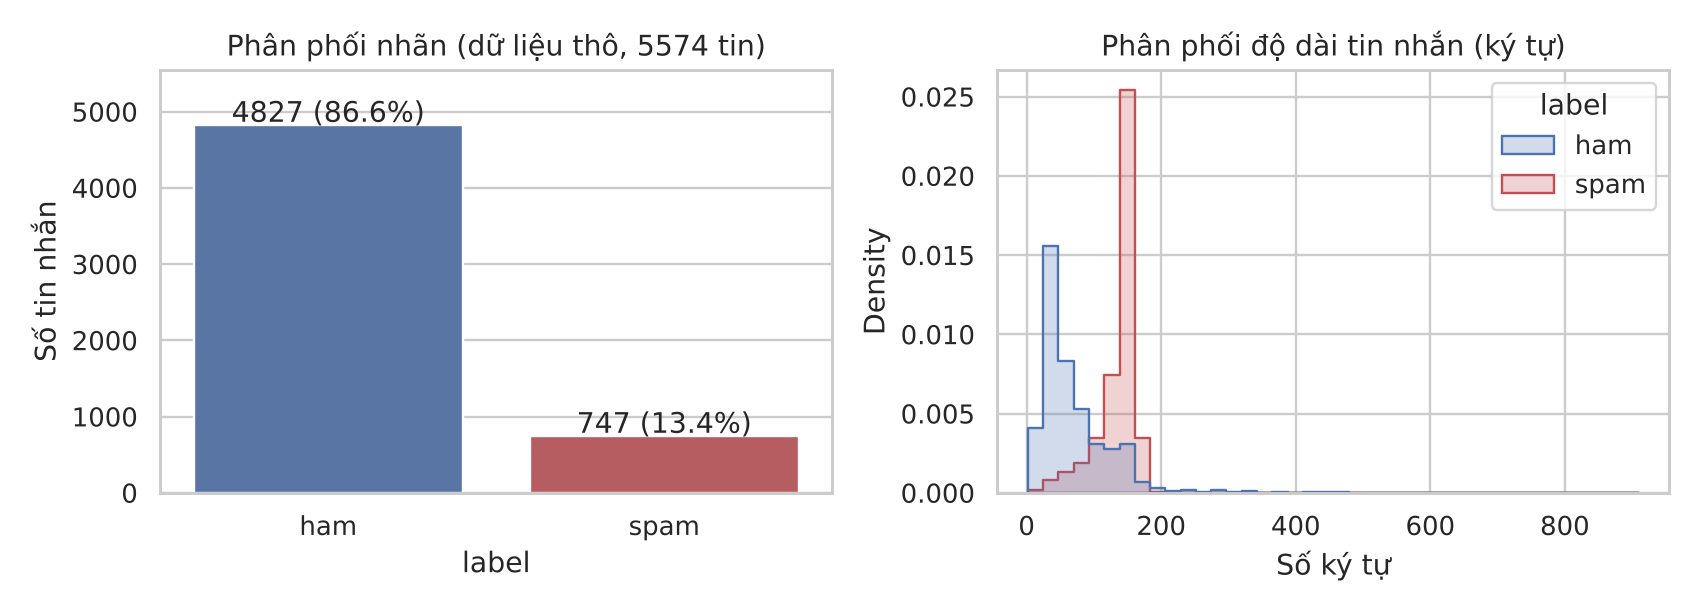
\includegraphics[width=0.95\textwidth]{images/eda_label_length.png}
    \caption{Phân phối nhãn dữ liệu thô (trái) và biểu đồ phân phối độ dài tin nhắn theo lớp (phải)}
    \label{fig:eda-label-length}
    \Nguon{Trích xuất tự động từ module thực nghiệm run\_experiments.py}
\end{figure}

Sự mất cân bằng này dẫn tới một hệ quả toán học và phương pháp luận cực kỳ quan trọng:
\begin{itemize}
    \item Giả sử xây dựng một bộ phân loại mù mờ (Naive Dummy Classifier) luôn luôn đưa ra kết quả dự đoán là \texttt{ham} cho mọi tin nhắn mà không cần đọc nội dung, bộ phân loại này vẫn đạt được độ chính xác (Accuracy) lên tới \textbf{87,4\%} trên tập huấn luyện và \textbf{87,3\%} trên tập kiểm thử!
    \item Tuy nhiên, một mô hình như vậy hoàn toàn vô dụng trong thực tiễn vì tỷ lệ bỏ sót tin nhắn rác là 100\% (Recall của spam bằng 0).
    \item Do đó, nhóm đi đến kết luận phương pháp luận cốt lõi: \textbf{Tuyệt đối không sử dụng độ chính xác (Accuracy) làm độ đo duy nhất hoặc tiêu chí chính để tối ưu hóa và so sánh mô hình}. Thay vào đó, nhóm thiết lập chỉ số F1-score của lớp dương (Spam) cùng với Precision, Recall, ma trận nhầm lẫn và diện tích dưới đường cong ROC (ROC-AUC) làm các thước đo trung tâm để đánh giá chất lượng mô hình.
\end{itemize}

\subsection{Phân tích đặc trưng hình thái và tín hiệu cấu trúc văn bản}
Để tìm kiếm các đặc trưng có khả năng phân biệt mạnh giữa hai lớp, nhóm đã tiến hành phân tích sâu về hình thái văn bản, độ dài tin nhắn và tần suất xuất hiện của các thành phần phi từ ngữ.
Các chỉ số thống kê mô tả được tổng hợp chi tiết trong Bảng~\ref{tab:tin-hieu-cau-truc}.

\begin{table}[H]
\centering
\caption{Đặc trưng hình thái và tỷ lệ xuất hiện các tín hiệu cấu trúc giữa hai lớp}
\label{tab:tin-hieu-cau-truc}
\begin{tabular}{|l|c|c|l|}
\hline
\textbf{Đặc trưng thống kê} & \textbf{Tin hợp lệ (Ham)} & \textbf{Tin rác (Spam)} & \textbf{Nhận xét phân hóa} \\
\hline
Độ dài trung bình (ký tự) & 70,9 & 137,7 & Spam dài gấp đôi Ham \\
\hline
Độ dài trung vị (ký tự) & 53,0 & 148,0 & Spam tập trung sát ngưỡng 160 \\
\hline
Độ dài lớn nhất (ký tự) & 910,0 & 223,0 & Ham có đuôi dài do viết tự do \\
\hline
Số lượng từ trung bình & 14,2 & 23,7 & Spam có mật độ từ ngữ cao hơn \\
\hline
Chứa chuỗi số dài ($\ge 5$ chữ số) & 0,1\% & 76,7\% & Tín hiệu phân biệt cực kỳ mạnh \\
\hline
Chứa địa chỉ web hoặc tên miền (URL) & 0,3\% & 17,8\% & Tỷ lệ xuất hiện ở Spam gấp 59 lần \\
\hline
Chứa ký hiệu tiền tệ (£, \$, €) & 0,4\% & 33,2\% & Tỷ lệ xuất hiện ở Spam gấp 83 lần \\
\hline
Tỷ lệ ký tự viết HOA trung bình & 7,7\% & 16,6\% & Spam lạm dụng chữ hoa để gây chú ý \\
\hline
\end{tabular}
\Nguon{Trích xuất tự động từ module run\_experiments.py}
\end{table}

Từ biểu đồ phân phối tại Hình~\ref{fig:eda-label-length} và các chỉ số trong Bảng~\ref{tab:tin-hieu-cau-truc}, nhóm rút ra các quan sát sâu sắc sau:
\begin{enumerate}
    \item \textbf{Về độ dài văn bản:} Các tin nhắn hợp lệ (\texttt{ham}) mang tính chất đối thoại thường nhật, thường rất ngắn gọn (trung vị chỉ 53 ký tự, 11 từ), nhưng phân phối có độ lệch phải rất lớn với một số tin nhắn dài tới 910 ký tự. Ngược lại, tin nhắn rác (\texttt{spam}) có phân phối độ dài rất tập trung quanh ngưỡng 130 đến 160 ký tự (trung bình 137,7 ký tự, trung vị 148 ký tự). Điều này phản ánh rõ nét thói quen của các đối tượng phát tán tin rác: cố gắng tận dụng tối đa giới hạn 160 ký tự của một bản tin SMS tiêu chuẩn để truyền tải càng nhiều thông tin quảng cáo, mời chào càng tốt.
    \item \textbf{Về tín hiệu chuỗi số dài (Long numeric sequences):} Có tới \textbf{76,7\%} tin nhắn rác chứa các chuỗi số từ 5 chữ số liên tiếp trở lên (đại diện cho số điện thoại hotline, đầu số tổng đài nhắn tin trả thưởng hoặc mã dịch vụ), trong khi ở tin nhắn thông thường tỷ lệ này chỉ là \textbf{0,1\%} (chênh lệch tới hơn 760 lần).
    \item \textbf{Về tín hiệu địa chỉ web (URL) và tiền tệ (Currency):} Tin nhắn rác xuất hiện dày đặc các ký hiệu tiền tệ (£, \$, €) chiếm 33,2\% (so với 0,4\% ở tin thường) và các đường dẫn website hoặc tên miền chiếm 17,8\% (so với 0,3\% ở tin thường).
    \item \textbf{Về phong cách biểu cảm:} Tin nhắn rác có tỷ lệ ký tự viết hoa trung bình lên tới 16,6\% (gấp hơn 2 lần tin thường), do các đối tượng gửi tin rác cố tình sử dụng các từ viết hoa toàn bộ như *“WINNER”*, *“FREE”*, *“URGENT”*, *“CLAIM NOW”* nhằm kích thích thị giác và thao túng tâm lý người nhận.
\end{enumerate}

\subsection{Khảo sát phân phối từ vựng đặc trưng theo lớp}
Bên cạnh các đặc trưng cấu trúc bề mặt, nhóm đã phân tích phân phối tần suất của các từ vựng xuất hiện nhiều nhất trong từng lớp (sau khi áp dụng chuẩn hóa và loại bỏ từ dừng tiếng Anh). Kết quả được trực quan hóa tại Hình~\ref{fig:eda-top-words}.

\begin{figure}[H]
    \centering
    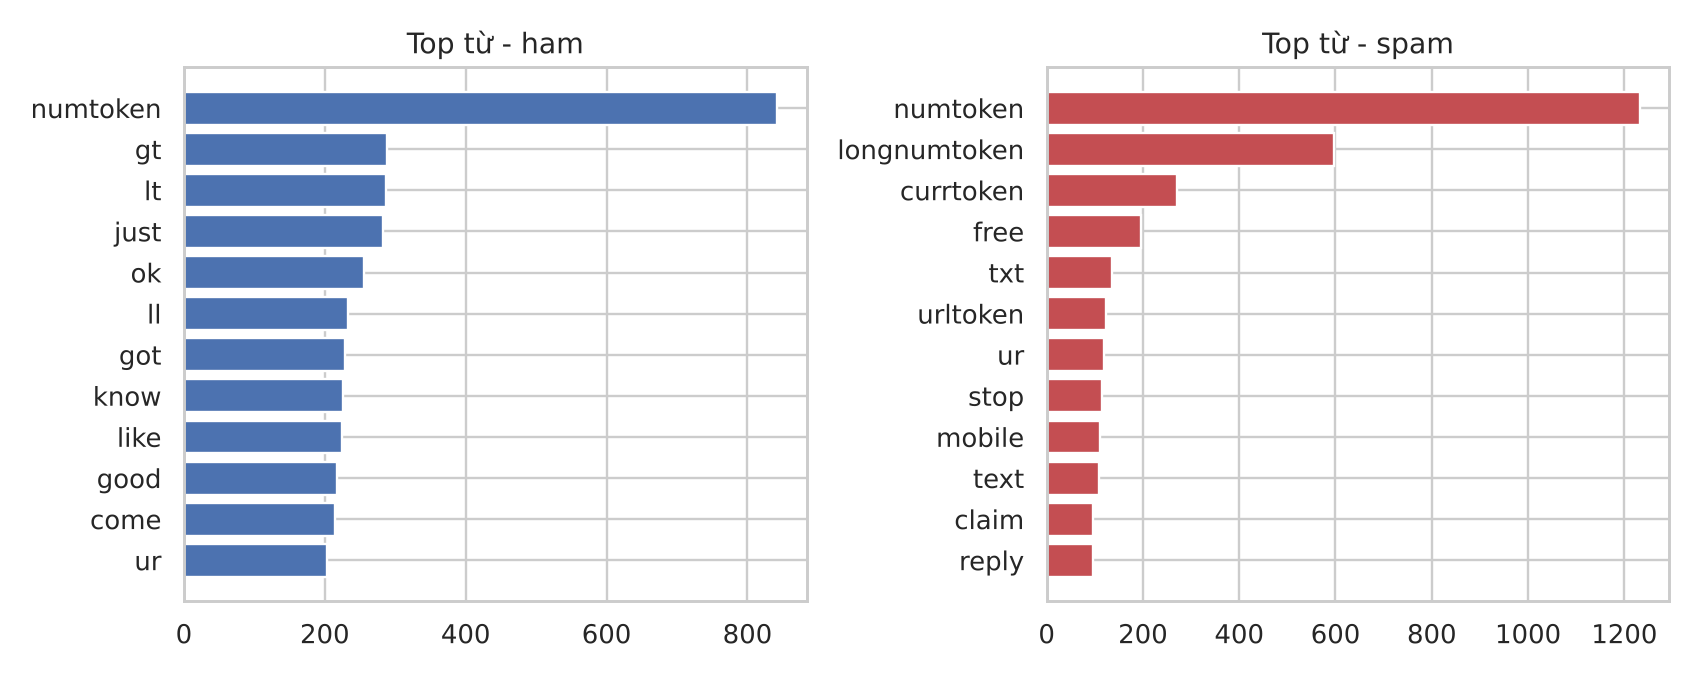
\includegraphics[width=0.9\textwidth]{images/eda_top_words.png}
    \caption{Top các từ vựng xuất hiện nhiều nhất trong lớp tin hợp lệ (trái) và lớp tin nhắn rác (phải)}
    \label{fig:eda-top-words}
    \Nguon{Trích xuất tự động từ module run\_experiments.py}
\end{figure}

Phân tích Hình~\ref{fig:eda-top-words} cho thấy sự phân cực từ vựng sâu sắc giữa hai thế giới văn bản:
\begin{itemize}
    \item \textbf{Thế giới của tin nhắn hợp lệ (Ham):} Bị chi phối bởi các từ ngữ giao tiếp thường nhật, chỉ địa điểm, thời gian, hoạt động cá nhân và cảm xúc thân mật: \texttt{home}, \texttt{come}, \texttt{later}, \texttt{ok}, \texttt{good}, \texttt{like}, \texttt{know}, \texttt{love}, \texttt{going}. Đặc biệt, xuất hiện hai token \texttt{gt} và \texttt{lt} với tần suất rất cao (nhóm sẽ phân tích nguyên nhân kỹ thuật của hiện tượng này ở Chương~\ref{chap:chuong5}).
    \item \textbf{Thế giới của tin nhắn rác (Spam):} Bị chi phối hoàn toàn bởi các thuật ngữ tiếp thị, tài chính, mệnh lệnh hành động và hứa hẹn lợi ích: \texttt{free}, \texttt{txt}, \texttt{claim}, \texttt{prize}, \texttt{won}, \texttt{mobile}, \texttt{urgent}, \texttt{cash}, \texttt{reply}, \texttt{contact}.
\end{itemize}

\section{Thiết lập hệ giả thuyết nghiên cứu}
\label{sec:gia-thuyet}

Dựa trên các bằng chứng định lượng thu nhận được từ quá trình khám phá dữ liệu (EDA), nhóm chính thức thiết lập hệ thống ba giả thuyết nghiên cứu (Research Hypotheses) làm kim chỉ nam xuyên suốt toàn bộ quá trình thiết kế giải pháp và thực nghiệm mô hình:

\begin{itemize}
    \item \textbf{Giả thuyết H1 (Bảo toàn tín hiệu cấu trúc qua kỹ thuật gom token đặc biệt):}
    \textit{“Do các chuỗi số điện thoại cụ thể, đường dẫn URL hoặc giá trị tiền tệ cụ thể hiếm khi lặp lại y hệt giữa các tin nhắn (tạo ra các từ vựng thưa thớt, vô nghĩa nếu để nguyên), việc áp dụng biểu thức chính quy (Regex) để quy đổi toàn bộ các thực thể này về các token tín hiệu chung có chủ đích (như \texttt{longnumtoken}, \texttt{urltoken}, \texttt{currtoken}, \texttt{numtoken}) sẽ giữ lại triệt để thông tin ngữ nghĩa then chốt, giúp cải thiện rõ rệt hiệu năng của các mô hình phân loại (đặc biệt là Cây quyết định và Naive Bayes) so với phương án xử lý thô hoặc xóa bỏ ký tự đặc biệt một cách máy móc.”}
    
    \item \textbf{Giả thuyết H2 (Hiệu quả của không gian n-gram kết hợp unigram và bigram):}
    \textit{“Các cụm từ cố định trong tin nhắn rác thường xuất hiện dưới dạng các cụm 2 từ có tính cảnh báo cao (ví dụ: *“cash prize”*, *“claim now”*, *“urgent call”*). Do đó, việc mở rộng không gian biểu diễn từ unigram đơn thuần sang kết hợp unigram + bigram sẽ giúp mô hình học được mối liên kết ngữ cảnh cục bộ, từ đó nâng cao độ chính xác nhận diện tin nhắn rác.”}
    
    \item \textbf{Giả thuyết H3 (Tầm quan trọng của cân đối chi phí lỗi và tiêu chí tối ưu hóa F1):}
    \textit{“Trong bài toán thực tế, chi phí của lỗi Dương tính giả (FP --- chặn nhầm một tin nhắn công việc hay giao dịch quan trọng) gây tổn thất lớn hơn rất nhiều so với lỗi Âm tính giả (FN --- để lọt một tin nhắn rác vào hòm thư). Do đó, việc tối ưu hóa siêu tham số bằng Cross-Validation cần căn cứ trên độ đo F1-score của lớp spam kết hợp giám sát chặt chẽ Precision, thay vì tối ưu hóa theo Accuracy thuần túy.”}
\end{itemize}

\section{Tóm tắt chương 1}
Chương 1 đã thiết lập toàn diện bức tranh tổng quan của đề tài nghiên cứu. Bộ dữ liệu SMS Spam Collection gồm 5.574 tin nhắn đã được làm sạch, loại bỏ 403 mẫu trùng lặp nhằm triệt tiêu nguy cơ rò rỉ dữ liệu, còn lại 5.171 mẫu duy nhất. Quá trình EDA đã chứng minh tính chất mất cân bằng nhãn sâu sắc (12,6\% spam) và nhận diện được các tín hiệu cấu trúc mang tính bản chất: tin nhắn rác dài hơn rõ rệt, chứa tới 76,7\% chuỗi số dài, 33,2\% ký hiệu tiền tệ và 17,8\% liên kết web. Hệ giả thuyết H1, H2, H3 được xác lập sẽ là nền tảng định hướng cho toàn bộ các bước thiết kế lý thuyết, xây dựng pipeline và thử nghiệm mô hình trong các chương tiếp theo.